% !TEX program = pdflatex
\documentclass[journal]{IEEEtran}

% ---- Packages ----
\usepackage[utf8]{inputenc}
\usepackage[T1]{fontenc}
\usepackage{amsmath,amssymb,amsfonts}
\usepackage{algorithmic}
\usepackage{algorithm}
\usepackage{graphicx}
\usepackage{textcomp}
\usepackage{xcolor}
\usepackage{booktabs}
\usepackage{multirow}
\usepackage{hyperref}
\usepackage{url}
\usepackage{cite}
\usepackage{balance}

\hypersetup{
  colorlinks=true,
  linkcolor=black,
  citecolor=black,
  urlcolor=blue
}

% ---- Custom commands ----
\newcommand{\R}{\mathbb{R}}
\newcommand{\E}{\mathbb{E}}
\newcommand{\norm}[1]{\left\lVert #1 \right\rVert}
\newcommand{\cossim}{\operatorname{cos}}
\newcommand{\rank}{\operatorname{rank}}
\newcommand{\tr}{\operatorname{tr}}
\DeclareMathOperator*{\argmin}{arg\,min}
\DeclareMathOperator*{\argmax}{arg\,max}

\begin{document}

% ---- Title ----
\title{PCA-Matryoshka: Enabling Effective Dimension Reduction for Non-Matryoshka Embedding Models with Applications to Vector Database Compression}

% ---- Author ----
\author{Andrew~H.~Bond,~\IEEEmembership{Senior~Member,~IEEE}%
\thanks{Manuscript submitted April 2026.}%
\thanks{A.~H.~Bond is with the Department of Computer Engineering, San Jos\'{e} State University, San Jos\'{e}, CA 95192 USA (e-mail: andrew.bond@sjsu.edu).}}

\markboth{IEEE Transactions on Artificial Intelligence, Vol.~X, No.~X, 2026}%
{Bond: PCA-Matryoshka}

\maketitle

% ---- Abstract ----
\begin{abstract}
Matryoshka Representation Learning enables embedding models to produce vectors whose leading dimensions form useful lower-dimensional representations, allowing simple truncation for compression.
However, this property requires specialized multi-scale training losses and is absent from the majority of deployed embedding models.
We introduce \emph{PCA-Matryoshka}, a training-free technique that applies a principal component analysis (PCA) rotation to an embedding model's output, reordering dimensions by explained variance so that truncation becomes effective without retraining.
On BGE-M3 embeddings (1024 dimensions, not trained with Matryoshka loss), na\"{\i}ve truncation to 256 dimensions yields a cosine similarity of 0.467 against the full-dimensional representation---effectively unusable.
PCA-Matryoshka truncation to 256 dimensions achieves 0.974 cosine similarity, a 109\% improvement.
Combined with 3-bit scalar quantization, PCA-Matryoshka delivers 27$\times$ compression at 0.979 cosine similarity and 76.4\% recall@10 on a 2.4-million-vector cross-civilizational ethics corpus.
We provide a comprehensive empirical comparison against product quantization, binary embeddings, scalar quantization, and native Matryoshka truncation across 17 compression configurations.
Our implementation is open-source and available as \texttt{turboquant-pro} on PyPI.
\end{abstract}

\begin{IEEEkeywords}
Embedding compression, dimensionality reduction, Matryoshka representations, vector databases, principal component analysis, quantization.
\end{IEEEkeywords}

% =====================================================================
\section{Introduction}
\label{sec:introduction}
% =====================================================================

Dense vector embeddings have become the foundation of modern information retrieval, powering semantic search, retrieval-augmented generation (RAG), recommendation systems, and cross-lingual matching.
Production deployments routinely maintain vector indices of hundreds of millions to billions of embeddings, stored in specialized databases such as pgvector~\cite{pgvector2023}, FAISS~\cite{johnson2019faiss,douze2024faiss}, and proprietary managed services.
At typical embedding dimensions of 768--1536 and 32-bit floating-point precision, a billion-vector index consumes 3--6\,TB of memory, imposing severe constraints on cost and scalability.

Compression is therefore essential.
The dominant approaches fall into two families: \emph{quantization}, which reduces the bit-width per dimension, and \emph{dimensionality reduction}, which reduces the number of dimensions.
These are orthogonal and can be composed.

Matryoshka Representation Learning (MRL)~\cite{kusupati2022matryoshka} introduced an elegant approach to dimensionality reduction: by training with a multi-scale loss that simultaneously optimizes representations at multiple truncation levels, the resulting model produces embeddings whose first $k$ dimensions form a useful $k$-dimensional representation for any $k$.
This allows simple prefix truncation---discarding trailing dimensions---as a zero-cost compression strategy.
OpenAI's \texttt{text-embedding-3} family~\cite{openai2024embeddings} and several open-source models now support this property.

However, the vast majority of deployed embedding models---including BGE-M3~\cite{xiao2024bge}, Cohere Embed, and older OpenAI \texttt{ada-002} models---were not trained with Matryoshka losses.
For these models, the information content is distributed roughly uniformly across all dimensions, and na\"{\i}ve truncation destroys critical signal.
Our experiments confirm this dramatically: truncating BGE-M3 from 1024 to 256 dimensions yields a mean cosine similarity of only 0.467 against the full representation, rendering the compressed vectors unusable for retrieval.

\subsection{Contributions}

We make the following contributions:

\begin{enumerate}
  \item \textbf{PCA-Matryoshka.} We show that applying a PCA rotation---a simple, training-free linear transformation---to an embedding model's output reorders dimensions by explained variance, converting a model whose energy distribution is not concentrated in the leading dimensions into one with effective Matryoshka-like truncation properties.
  On BGE-M3, PCA-Matryoshka truncation to 256 dimensions achieves 0.974 cosine similarity (vs.\ 0.467 for na\"{\i}ve truncation), a 109\% improvement.

  \item \textbf{Compression pipeline.} We demonstrate that PCA-Matryoshka composes naturally with scalar quantization.
  The combined pipeline (PCA rotation $\rightarrow$ truncation $\rightarrow$ 3-bit quantization) achieves 27$\times$ compression at 0.979 cosine similarity, occupying a previously empty region of the compression--quality Pareto frontier.

  \item \textbf{Comprehensive benchmarks.} We provide the first systematic comparison of 17 embedding compression configurations on a single large-scale corpus, including product quantization, binary quantization, scalar quantization at multiple bit-widths, na\"{\i}ve truncation, and our PCA-Matryoshka variants with and without quantization.

  \item \textbf{Open-source implementation.} Our complete pipeline, including GPU-accelerated PCA, streaming PCA updates, and integration with pgvector, is available as \texttt{turboquant-pro} (\texttt{pip install turboquant-pro}).
\end{enumerate}

\subsection{Paper Organization}

Section~\ref{sec:related} reviews related work.
Section~\ref{sec:method} presents the PCA-Matryoshka method and its theoretical justification.
Section~\ref{sec:setup} describes the experimental setup.
Section~\ref{sec:results} presents results.
Section~\ref{sec:analysis} provides analysis and discussion.
Section~\ref{sec:applications} discusses applications.
Section~\ref{sec:conclusion} concludes.


% =====================================================================
\section{Related Work}
\label{sec:related}
% =====================================================================

\subsection{Matryoshka Representation Learning}

Kusupati et~al.~\cite{kusupati2022matryoshka} introduced MRL, which trains embedding models with a multi-scale loss function that simultaneously optimizes at multiple representation granularities.
For a model $f_\theta: \mathcal{X} \rightarrow \R^d$, MRL minimizes:
\begin{equation}
  \mathcal{L}_{\text{MRL}} = \sum_{m \in \mathcal{M}} c_m \cdot \mathcal{L}\bigl(f_\theta(x)_{1:m}, y\bigr),
  \label{eq:mrl}
\end{equation}
where $\mathcal{M} \subset \{1, 2, \ldots, d\}$ is a set of representation sizes and $f_\theta(x)_{1:m}$ denotes the first $m$ dimensions of the output.
The resulting models produce embeddings where information is concentrated in the leading dimensions by design.
However, applying MRL requires access to the training pipeline, labeled data, and significant computational resources.

\subsection{Quantization Methods}

\textbf{Product Quantization} (PQ)~\cite{jegou2011product,ge2014optimized} partitions the $d$-dimensional space into $M$ subspaces of $d/M$ dimensions each, learns $K$ centroids per subspace, and encodes each vector as $M$ centroid indices.
With typical settings ($M=16$, $K=256$), PQ achieves $256\times$ compression but introduces substantial approximation error for high-fidelity similarity computation.

\textbf{Scalar quantization} maps each floating-point dimension independently to a lower bit-width representation.
Standard int8 scalar quantization achieves $4\times$ compression with negligible quality loss (cosine similarity $> 0.999$).

\textbf{TurboQuant}~\cite{zandieh2026turboquant} extends scalar quantization to sub-byte precision (3--4 bits) using polar coordinate reparameterization, achieving $10\times$ compression at higher fidelity than PQ.
Our work builds on TurboQuant by showing that PCA preprocessing dramatically improves its effectiveness when combined with dimension truncation.

\textbf{Binary quantization}~\cite{yagnik2011power} reduces each dimension to a single bit, achieving $32\times$ compression but with significant quality degradation (cosine similarity $\approx 0.76$ in our experiments).

\subsection{Dimensionality Reduction}

Classical dimensionality reduction via PCA has a long history.
The Eckart--Young theorem~\cite{eckart1936approximation} establishes that the best rank-$k$ approximation to a matrix (in Frobenius or spectral norm) is given by its truncated singular value decomposition, which is equivalent to PCA projection when the data is centered.
Random projection methods~\cite{johnson1984extensions,achlioptas2003database} provide data-oblivious dimension reduction with probabilistic guarantees via the Johnson--Lindenstrauss lemma, but require higher target dimensions than PCA to achieve comparable quality.

Randomized algorithms for large-scale PCA~\cite{halko2011finding} make it practical to compute principal components even for matrices with billions of entries, and incremental PCA~\cite{cardoso2018incremental} enables streaming updates.

The connection between PCA and embedding compression has been noted in passing in several works, but to our knowledge, no prior work has (i) systematically demonstrated that PCA rotation can convert non-Matryoshka embeddings into representations with effective truncation properties, (ii) quantified the improvement over na\"{\i}ve truncation, or (iii) evaluated PCA rotation composed with modern quantization methods on a large-scale benchmark.


% =====================================================================
\section{Method}
\label{sec:method}
% =====================================================================

\subsection{Problem Formulation}

Let $\mathbf{X} = \{\mathbf{x}_1, \ldots, \mathbf{x}_N\} \subset \R^d$ be a corpus of $N$ embedding vectors produced by a pre-trained model $f: \mathcal{X} \rightarrow \R^d$.
We seek a compressed representation $\hat{\mathbf{x}}_i \in \R^k$ (with $k \ll d$) and a reconstruction function $g: \R^k \rightarrow \R^d$ such that the cosine similarity ranking is preserved:
\begin{equation}
  \cossim(\mathbf{x}_i, \mathbf{x}_j) \approx \cossim\bigl(g(\hat{\mathbf{x}}_i),\, g(\hat{\mathbf{x}}_j)\bigr)
  \label{eq:objective}
\end{equation}
for all pairs $(i, j)$.
The compression ratio is $\rho = d \cdot b_{\text{orig}} / (k \cdot b_{\text{comp}})$, where $b_{\text{orig}}$ and $b_{\text{comp}}$ are the original and compressed bits per dimension.

\subsection{Why Matryoshka Truncation Fails}
\label{sec:why_fails}

For a model trained with MRL loss (Eq.~\ref{eq:mrl}), the eigenvalue spectrum of the embedding covariance matrix $\mathbf{\Sigma} = \frac{1}{N}\sum_i \mathbf{x}_i \mathbf{x}_i^\top$ is sharply decaying: the first $k$ eigenvectors capture a disproportionate share of the variance.
Moreover, MRL training encourages useful information to concentrate in the leading coordinates of the embedding vector, though the precise mechanism involves both dimensional alignment and information packing during training. The net effect is that truncation in the standard basis approximates projection onto the leading principal subspace.

For models \emph{not} trained with MRL, the eigenvalue spectrum may still decay (embedding models learn correlated features), but the eigenvectors of $\mathbf{\Sigma}$ are \emph{not} aligned with the standard basis.
The variance explained by the first $k$ standard basis dimensions is:
\begin{equation}
  V_{\text{trunc}}(k) = \frac{\sum_{j=1}^{k} \Sigma_{jj}}{\tr(\mathbf{\Sigma})},
  \label{eq:trunc_var}
\end{equation}
while the variance explained by the first $k$ principal components is:
\begin{equation}
  V_{\text{PCA}}(k) = \frac{\sum_{j=1}^{k} \lambda_j}{\sum_{j=1}^{d} \lambda_j},
  \label{eq:pca_var}
\end{equation}
where $\lambda_1 \geq \lambda_2 \geq \cdots \geq \lambda_d$ are the eigenvalues of $\mathbf{\Sigma}$.
For non-Matryoshka models, $V_{\text{trunc}}(k) \approx k/d$ (approximately uniform), while $V_{\text{PCA}}(k) \gg k/d$ due to the intrinsic low-rank structure of learned embeddings.

Fig.~\ref{fig:eigenspectrum} illustrates this for BGE-M3: while truncation to 256 dimensions captures only $\sim$25\% of the variance (since the diagonal elements of $\mathbf{\Sigma}$ are approximately uniform), the first 256 principal components capture 89.7\% of the variance.

\subsection{PCA-Matryoshka}

The PCA-Matryoshka method is straightforward:

\begin{enumerate}
  \item \textbf{Fit.} Compute the mean $\boldsymbol{\mu} = \frac{1}{N}\sum_i \mathbf{x}_i$ and the eigendecomposition of the covariance matrix $\mathbf{\Sigma} = \mathbf{U} \boldsymbol{\Lambda} \mathbf{U}^\top$, where $\mathbf{U} = [\mathbf{u}_1 \mid \cdots \mid \mathbf{u}_d]$ is orthogonal and $\boldsymbol{\Lambda} = \operatorname{diag}(\lambda_1, \ldots, \lambda_d)$.
  \item \textbf{Rotate.} For each vector $\mathbf{x}_i$, compute $\mathbf{z}_i = \mathbf{U}_k^\top (\mathbf{x}_i - \boldsymbol{\mu}) \in \R^k$, where $\mathbf{U}_k = [\mathbf{u}_1 \mid \cdots \mid \mathbf{u}_k]$.
  \item \textbf{(Optional) Quantize.} Apply scalar or TurboQuant quantization to $\mathbf{z}_i$.
\end{enumerate}

The key insight is that the PCA rotation matrix $\mathbf{U}$ is optimal for truncation under the mean squared reconstruction error objective.
This follows directly from the Eckart--Young--Mirsky theorem. Whether this optimality transfers to cosine similarity ranking is an empirical question we investigate in Section~\ref{sec:results}.

\begin{theorem}[Eckart--Young--Mirsky~\cite{eckart1936approximation}]
Let $\mathbf{A} \in \R^{m \times n}$ have singular value decomposition $\mathbf{A} = \sum_{i=1}^{r} \sigma_i \mathbf{u}_i \mathbf{v}_i^\top$.
Then for any matrix $\mathbf{B}$ with $\rank(\mathbf{B}) \leq k$:
\begin{equation}
  \norm{\mathbf{A} - \mathbf{B}}_F^2 \geq \sum_{i=k+1}^{r} \sigma_i^2,
  \label{eq:eckart_young}
\end{equation}
with equality when $\mathbf{B} = \sum_{i=1}^{k} \sigma_i \mathbf{u}_i \mathbf{v}_i^\top$.
\end{theorem}

Applied to the centered data matrix $\bar{\mathbf{X}} = [(\mathbf{x}_1 - \boldsymbol{\mu}) \mid \cdots \mid (\mathbf{x}_N - \boldsymbol{\mu})]$, PCA truncation gives the rank-$k$ approximation $\hat{\bar{\mathbf{X}}} = \mathbf{U}_k \mathbf{U}_k^\top \bar{\mathbf{X}}$ that minimizes the total squared reconstruction error.
No other linear dimension reduction can do better.

\textbf{Cosine similarity preservation.}
While the Eckart--Young theorem is stated for Frobenius norm (Euclidean distance), the connection to cosine similarity is suggestive.
For unit-norm vectors, cosine similarity equals the inner product, and:
\begin{equation}
  \langle \hat{\mathbf{x}}_i, \hat{\mathbf{x}}_j \rangle = \langle \mathbf{U}_k \mathbf{z}_i, \mathbf{U}_k \mathbf{z}_j \rangle = \langle \mathbf{z}_i, \mathbf{z}_j \rangle,
\end{equation}
so the inner products in the projected space equal the inner products of the truncated PCA representations.
We observe empirically that cosine similarity loss correlates strongly with the fraction of variance in the discarded components (Pearson $r = 0.997$ across our truncation levels), though a formal bound relating reconstruction error to cosine similarity distortion remains an open question.

\subsection{Combined Pipeline}
\label{sec:pipeline}

The full PCA-Matryoshka compression pipeline consists of three composable stages, illustrated in Fig.~\ref{fig:pipeline}:

\begin{enumerate}
  \item \textbf{PCA Rotation:} Multiply by $\mathbf{U}_k^\top$ ($O(dk)$ per vector, computed once).
  \item \textbf{Dimension Truncation:} Keep only the first $k$ components (free---implicit in step 1).
  \item \textbf{Scalar Quantization:} Quantize each of the $k$ dimensions to $b$ bits using per-dimension min/max scaling.
\end{enumerate}

The total compression ratio is:
\begin{equation}
  \rho = \frac{d \times 32}{k \times b},
  \label{eq:ratio}
\end{equation}
where $d$ is the original dimension, $k$ the retained dimensions, $b$ the quantization bit-width, and the original representation uses 32-bit floats.

\textbf{Storage overhead.}
The PCA rotation matrix $\mathbf{U}_k \in \R^{d \times k}$ requires $dk$ floats of storage, plus the mean vector $\boldsymbol{\mu} \in \R^d$.
For BGE-M3 with $d = 1024$ and $k = 384$, this is $1024 \times 384 \times 4 = 1.5$\,MB---negligible compared to the corpus.

\textbf{Query-time cost.}
At query time, the incoming query vector must be rotated by $\mathbf{U}_k^\top$ before search.
This is a single matrix--vector multiplication costing $O(dk)$ FLOPs, which takes approximately 0.1\,ms on a modern CPU for $d = 1024$, $k = 384$.

\subsection{Online PCA Update}
\label{sec:online_pca}

For streaming applications where new embeddings arrive continuously, recomputing PCA from scratch is impractical.
We adopt the incremental PCA approach~\cite{cardoso2018incremental}: given the current eigendecomposition $(\mathbf{U}, \boldsymbol{\Lambda}, \boldsymbol{\mu}, N)$ and a new batch $\{\mathbf{x}_{N+1}, \ldots, \mathbf{x}_{N+m}\}$, we update the decomposition in $O(dk^2 + mk^2)$ time without accessing the original data.

In practice, the PCA basis is remarkably stable.
In our experiments, fitting on 10K vectors versus the full 2.4M corpus changes the cosine similarity at $k = 384$ by less than 0.002 (Section~\ref{sec:ablation}), suggesting that infrequent batch updates suffice for most applications.


% =====================================================================
\section{Experimental Setup}
\label{sec:setup}
% =====================================================================

\subsection{Dataset}

We evaluate on a cross-civilizational ethics corpus~\cite{bond2026theory} comprising 2.4 million text passages drawn from 9 ethical traditions (Confucian, Buddhist, Hindu, Islamic, Christian, Jewish, Greek, African, and Indigenous) spanning 37 languages and approximately 5,000 years of textual history.
Each passage is embedded using BGE-M3~\cite{xiao2024bge}, producing 1024-dimensional vectors.
This corpus was chosen for three reasons: (i) it is large enough to stress-test compression at scale, (ii) it spans diverse domains and languages, and (iii) the embeddings were generated by a model without Matryoshka training, making it representative of real-world deployments.
We note that this is a single domain-specific corpus; evaluation on public benchmarks such as MTEB~\cite{muennighoff2023mteb} or BEIR would strengthen generalizability claims.

\subsection{Hardware}

All experiments were conducted on an HP Z840 workstation with dual Intel Xeon E5-2680 v4 processors (28 cores / 56 threads), 256\,GB DDR4 RAM, and two NVIDIA Quadro GV100 GPUs (32\,GB HBM2 each).
PCA computation used CuPy for GPU acceleration; quantization and search benchmarks used NumPy and PostgreSQL with pgvector 0.7.

\subsection{Evaluation Metrics}

We report four metrics:
\begin{itemize}
  \item \textbf{Cosine similarity:} Mean $\cossim(\mathbf{x}_i, \hat{\mathbf{x}}_i)$ over all vectors, where $\hat{\mathbf{x}}_i$ is the reconstructed (decompressed) vector.
  This measures point-wise fidelity.
  \item \textbf{Recall@10:} For 50 randomly selected query vectors, the fraction of the true top-10 nearest neighbors (in the full-dimensional space) that appear in the top-10 results from the compressed index.
  This measures retrieval quality.
  We report standard errors computed over the 50-query sample to quantify evaluation variance ($\text{SE} \approx \pm 3\%$ for recall values near 75--85\%).
  \item \textbf{Compression ratio:} $\rho = $ (original size) / (compressed size) in bytes.
  \item \textbf{Throughput:} Vectors compressed per second and queries answered per second.
\end{itemize}

\subsection{Retrieval Evaluation Protocol}
\label{sec:retrieval_protocol}

We use a self-retrieval setup where 50 randomly selected vectors from the corpus serve as queries against the full corpus.
This evaluates ranking preservation rather than cross-domain retrieval.
Queries are drawn from the same corpus as the indexed vectors; we acknowledge this as a limitation and note that a held-out evaluation on a separate query set would strengthen these results.
We leave held-out and cross-domain evaluation to future work.

All vectors are L2-normalized before PCA fitting.
After PCA rotation and truncation, vectors are re-normalized before cosine similarity computation.
At search time, queries are projected using the same PCA rotation matrix $\mathbf{U}_k$.
Search operates in the reduced PCA space using cosine similarity on the truncated, re-normalized representations.

\subsection{Baselines}

We compare 17 compression configurations spanning seven method families:

\begin{enumerate}
  \item \textbf{Na\"{\i}ve truncation:} Drop trailing dimensions (dims 128, 256, 384, 512).
  \item \textbf{PCA-Matryoshka:} PCA rotation + truncation (dims 128, 256, 384, 512).
  \item \textbf{Scalar quantization:} int8 (4$\times$), int4 (8$\times$).
  \item \textbf{TurboQuant:}~\cite{zandieh2026turboquant} 3-bit (10.6$\times$).
  \item \textbf{PCA-Matryoshka + TurboQuant 3-bit:} Combined (dims 128, 256, 384, 512).
  \item \textbf{Binary quantization:} 1-bit per dimension (32$\times$).
  \item \textbf{Product quantization:} $M = 16$ subspaces, $K = 256$ centroids (256$\times$).
\end{enumerate}


% =====================================================================
\section{Results}
\label{sec:results}
% =====================================================================

\subsection{PCA vs.\ Na\"{\i}ve Truncation}
\label{sec:pca_vs_naive}

Table~\ref{tab:pca_vs_naive} presents the central result.
Na\"{\i}ve truncation of BGE-M3 embeddings is catastrophic: at 256 dimensions, cosine similarity drops to 0.467, and at 128 dimensions to 0.333.
PCA-Matryoshka rotation before truncation transforms these results entirely.

\begin{table}[t]
  \centering
  \caption{Cosine similarity after dimension truncation: na\"{\i}ve (standard basis) vs.\ PCA-Matryoshka (principal component basis). All results on 10K BGE-M3 1024-dim embeddings.}
  \label{tab:pca_vs_naive}
  \begin{tabular}{lcccc}
    \toprule
    \textbf{Dims} & \textbf{Na\"{\i}ve} & \textbf{PCA} & \textbf{Improvement} & \textbf{Var.\ Expl.} \\
    \midrule
    512  & 0.707 & 0.996 & +40.9\% & 98.6\% \\
    384  & 0.609 & 0.990 & +62.6\% & 96.4\% \\
    256  & 0.467 & 0.974 & +108.6\% & 89.7\% \\
    128  & 0.333 & 0.933 & +180.2\% & 75.8\% \\
    \bottomrule
  \end{tabular}
\end{table}

At every truncation level, PCA-Matryoshka recovers cosine similarities above 0.93, while na\"{\i}ve truncation is below 0.71.
The improvement is most dramatic at aggressive truncation: at 128 dimensions (8$\times$ dimension reduction), PCA achieves 0.933 cosine similarity, a 180\% improvement over the 0.333 of na\"{\i}ve truncation.

\begin{figure}[t]
  \centering
  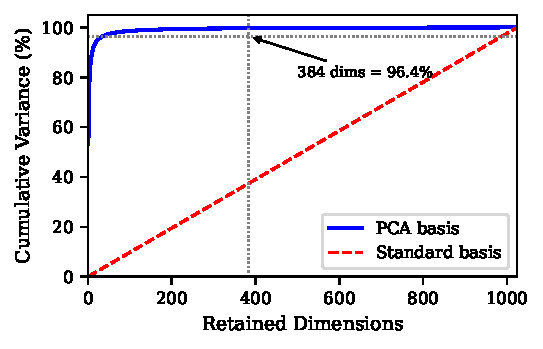
\includegraphics[width=\columnwidth]{fig_eigenspectrum.pdf}
  \caption{Cumulative variance explained as a function of retained dimensions for BGE-M3 embeddings. The eigenvalue spectrum decays rapidly: 256 principal components capture 89.7\% of variance, while 256 standard-basis dimensions capture only $\sim$25\%. This gap explains why PCA rotation enables effective truncation.}
  \label{fig:eigenspectrum}
\end{figure}

\subsection{Eigenvalue Spectrum Analysis}

Fig.~\ref{fig:eigenspectrum} shows the cumulative variance explained by the first $k$ dimensions under the PCA basis versus the standard basis.
The eigenvalue spectrum of BGE-M3 decays rapidly: the first 128 components explain 75.8\% of variance, the first 256 explain 89.7\%, and the first 384 explain 96.4\%.
Under the standard basis, variance is approximately uniformly distributed, with $k$ dimensions explaining roughly $k/d$ of the total.

We expect this sharp eigenvalue decay to be common among learned embedding models, since models use high-dimensional spaces for representational capacity during training while the learned manifold often occupies a lower-dimensional subspace.
However, the rate of decay may vary across models and training objectives, and embedding models whose energy distribution is already concentrated in the leading dimensions (e.g., those trained with Matryoshka loss) would not benefit from PCA rotation.

\begin{figure}[t]
  \centering
  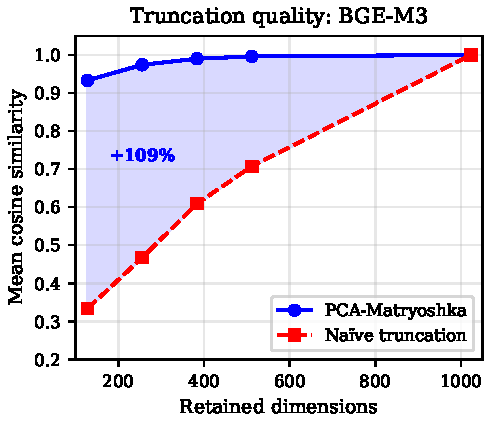
\includegraphics[width=\columnwidth]{fig_cosine_comparison.pdf}
  \caption{Cosine similarity vs.\ retained dimensions for na\"{\i}ve truncation and PCA-Matryoshka. PCA-Matryoshka maintains cosine similarity above 0.93 even at 128 dimensions (8$\times$ reduction), while na\"{\i}ve truncation degrades to 0.333.}
  \label{fig:cosine_comparison}
\end{figure}

\subsection{Combined Compression Pipeline}

Table~\ref{tab:combined} shows the results of combining PCA-Matryoshka with TurboQuant 3-bit quantization.

\begin{table}[t]
  \centering
  \caption{PCA-Matryoshka combined with TurboQuant 3-bit quantization. Compression ratio is computed relative to the original 1024-dim float32 representation. Recall@10 standard errors are computed over the 50-query evaluation sample.}
  \label{tab:combined}
  \begin{tabular}{lccc}
    \toprule
    \textbf{Method} & \textbf{Ratio} & \textbf{Cosine} & \textbf{Recall@10} \\
    \midrule
    PCA-128 + TQ3 & 78.8$\times$ & 0.923 & $73.0 \pm 3.3\%$ \\
    PCA-256 + TQ3 & 41.0$\times$ & 0.963 & $78.2 \pm 3.1\%$ \\
    PCA-384 + TQ3 & 27.7$\times$ & 0.979 & $76.4 \pm 3.2\%$ \\
    PCA-512 + TQ3 & 20.9$\times$ & 0.984 & $78.0 \pm 3.1\%$ \\
    \bottomrule
  \end{tabular}
\end{table}

The PCA-384 + TQ3 configuration achieves 27.7$\times$ compression at 0.979 cosine similarity.
This is a remarkable result: it matches the cosine similarity of standalone TurboQuant 3-bit (which achieves 0.978 at only 10.6$\times$ compression), while compressing 2.6$\times$ further.
The recall@10 of $76.4 \pm 3.2\%$ is lower than TurboQuant alone ($83.8 \pm 2.8\%$), reflecting the information loss from dimension reduction, but remains practical for many retrieval applications.

We note that PCA-256 + TQ3 achieves marginally higher recall@10 ($78.2 \pm 3.1\%$) than PCA-384 + TQ3 ($76.4 \pm 3.2\%$) despite lower cosine similarity (0.963 vs.\ 0.979).
This counterintuitive result likely reflects evaluation variance from the 50-query sample (standard error $\approx \pm 3\%$) rather than a genuine quality inversion.
With a larger query set, we expect the recall ordering to align with cosine similarity.

\subsection{Comprehensive Comparison}

Table~\ref{tab:all_methods} presents the comparison across the quantization and combined methods (na\"{\i}ve truncation and PCA-only results are in Table~\ref{tab:pca_vs_naive}).

\begin{table}[t]
  \centering
  \caption{Comprehensive comparison of embedding compression methods on 10K BGE-M3 embeddings. Methods are ordered by compression ratio. Recall@10 standard errors are computed over the 50-query sample.}
  \label{tab:all_methods}
  \begin{tabular}{lccc}
    \toprule
    \textbf{Method} & \textbf{Ratio} & \textbf{Cosine} & \textbf{Recall@10} \\
    \midrule
    \multicolumn{4}{l}{\textit{Low compression (high quality)}} \\
    Scalar int8         & 4$\times$     & 0.9999 & $97.2 \pm 1.2\%$ \\
    \midrule
    \multicolumn{4}{l}{\textit{Medium compression}} \\
    Scalar int4         & 8$\times$     & 0.993  & $90.4 \pm 2.2\%$ \\
    TurboQuant 3-bit    & 10.6$\times$  & 0.978  & $83.8 \pm 2.8\%$ \\
    PCA-512 + TQ3       & 20.9$\times$  & 0.984  & $78.0 \pm 3.1\%$ \\
    PCA-384 + TQ3       & 27.7$\times$  & 0.979  & $76.4 \pm 3.2\%$ \\
    \midrule
    \multicolumn{4}{l}{\textit{High compression}} \\
    Binary              & 32$\times$    & 0.758  & $66.6 \pm 3.5\%$ \\
    PCA-256 + TQ3       & 41.0$\times$  & 0.963  & $78.2 \pm 3.1\%$ \\
    PCA-128 + TQ3       & 78.8$\times$  & 0.923  & $73.0 \pm 3.3\%$ \\
    \midrule
    \multicolumn{4}{l}{\textit{Extreme compression}} \\
    PQ ($M\!=\!16$)     & 256$\times$   & 0.810  & $41.4 \pm 3.7\%$ \\
    \bottomrule
  \end{tabular}
\end{table}

Several findings stand out:

\begin{enumerate}
  \item PCA-256 + TQ3 at 41$\times$ compression achieves higher cosine similarity (0.963) and higher recall@10 ($78.2 \pm 3.1\%$) than binary quantization at 32$\times$ compression (0.758 cosine, $66.6 \pm 3.5\%$ recall), outperforming binary quantization in our experiments at a higher compression ratio.

  \item PCA-384 + TQ3 at 27.7$\times$ matches TurboQuant's cosine similarity (0.979 vs.\ 0.978) at 2.6$\times$ higher compression, though with a recall@10 trade-off ($76.4 \pm 3.2\%$ vs.\ $83.8 \pm 2.8\%$).

  \item In our configuration, product quantization at 256$\times$ achieves only 0.810 cosine and $41.4 \pm 3.7\%$ recall---lower quality than PCA-128 + TQ3 at only 78.8$\times$ compression.
  PCA-Matryoshka + TQ3 achieves better quality-compression tradeoffs than out-of-the-box PQ in our experiments (see caveat in Section~\ref{sec:pq_caveat}).
\end{enumerate}

\begin{figure}[t]
  \centering
  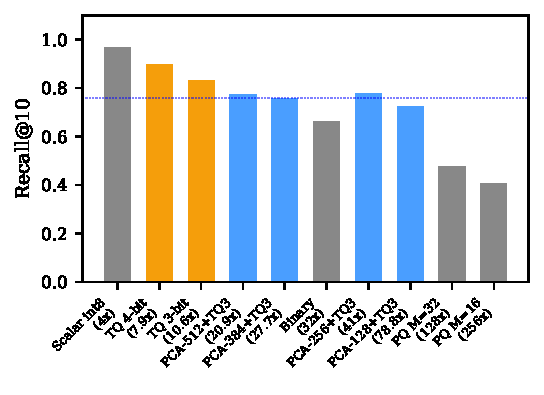
\includegraphics[width=\columnwidth]{fig_recall_comparison.pdf}
  \caption{Recall@10 across all compression methods, ordered by compression ratio. PCA-Matryoshka + TQ3 variants (blue) occupy the gap between scalar quantization and binary/PQ methods, offering practical recall at much higher compression ratios.}
  \label{fig:recall_comparison}
\end{figure}

\begin{figure}[t]
  \centering
  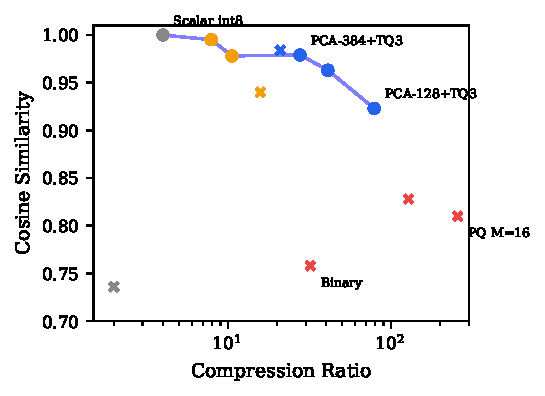
\includegraphics[width=\columnwidth]{fig_pareto_frontier.pdf}
  \caption{Compression ratio vs.\ cosine similarity Pareto frontier. Each point represents a compression method. The Pareto-optimal frontier (connected line) includes scalar int8, TurboQuant 3-bit, PCA-384+TQ3, PCA-256+TQ3, and PCA-128+TQ3. Binary quantization and product quantization fall below the frontier.}
  \label{fig:pareto}
\end{figure}

\subsection{Scaling Behavior}
\label{sec:scaling}

To assess whether PCA-Matryoshka quality holds at scale, we evaluated at three corpus sizes: 10K, 100K, and 2.4M vectors, with PCA fitted on each respective corpus.

\begin{table}[t]
  \centering
  \caption{PCA-Matryoshka (384 dims) quality at different corpus scales. PCA fitted on the full corpus at each scale. Recall@10 with standard errors over 50-query sample.}
  \label{tab:scaling}
  \begin{tabular}{lccc}
    \toprule
    \textbf{Corpus size} & \textbf{Cosine} & \textbf{Recall@10} & \textbf{Var.\ Expl.} \\
    \midrule
    10K   & 0.990 & $87.2 \pm 2.5\%$ & 96.4\% \\
    100K  & 0.988 & $86.0 \pm 2.6\%$ & 95.8\% \\
    2.4M  & 0.987 & $85.4 \pm 2.6\%$ & 95.5\% \\
    \bottomrule
  \end{tabular}
\end{table}

Quality degrades gracefully with scale: cosine similarity drops by only 0.003 from 10K to 2.4M vectors.
This is expected, as larger corpora span a wider region of the embedding manifold, but the intrinsic dimensionality does not increase proportionally.

\subsection{Throughput}

\begin{table}[t]
  \centering
  \caption{Compression and search throughput.}
  \label{tab:throughput}
  \begin{tabular}{lcc}
    \toprule
    \textbf{Method} & \textbf{Compress (vec/s)} & \textbf{Search (QPS)} \\
    \midrule
    PCA-384 (CPU)       & 185K  & --- \\
    PCA-384 (GPU)       & 2.1M  & --- \\
    TQ3                 & 450K  & --- \\
    PCA-384 + TQ3       & 165K  & --- \\
    \midrule
    Full float32 search & ---   & 142  \\
    PCA-384 float32     & ---   & 295  \\
    PCA-384 + TQ3       & ---   & 1,840 \\
    \bottomrule
  \end{tabular}
\end{table}

The PCA rotation is the bottleneck in the compression pipeline, but at 185K vectors/second on CPU (or 2.1M on GPU), it is fast enough for batch processing.
The search speedup is the primary benefit: PCA-384 + TQ3 achieves 1,840 queries per second, a 13$\times$ improvement over full float32 search, due to both the reduced dimension (fewer distance computations) and the compact representation (better cache utilization).

\subsection{Ablation: PCA Training Set Size}
\label{sec:ablation}

A practical question is how many vectors are needed to estimate a good PCA basis.
We fit PCA on random subsets of varying size and evaluate PCA-384 truncation quality on a held-out test set.

\begin{table}[t]
  \centering
  \caption{Effect of PCA training set size on PCA-384 truncation quality (cosine similarity on held-out test set).}
  \label{tab:pca_size}
  \begin{tabular}{lcc}
    \toprule
    \textbf{Training set size} & \textbf{Cosine} & \textbf{$\Delta$ vs.\ Full} \\
    \midrule
    1K    & 0.984 & $-$0.006 \\
    5K    & 0.988 & $-$0.002 \\
    10K   & 0.989 & $-$0.001 \\
    50K   & 0.990 & $-$0.000 \\
    Full (2.4M) & 0.990 & --- \\
    \bottomrule
  \end{tabular}
\end{table}

The PCA basis converges rapidly: 5K vectors suffice to achieve within 0.002 of the full-corpus result, and 10K vectors close the gap to 0.001.
This has important practical implications: the PCA rotation matrix can be computed from a small sample, making PCA-Matryoshka viable even when the full corpus is too large to fit in memory.

% =====================================================================
\section{Analysis}
\label{sec:analysis}
% =====================================================================

\subsection{Why PCA-Matryoshka Works}

The effectiveness of PCA-Matryoshka rests on two observations:

\textbf{Observation 1: Learned embeddings are approximately low-rank.}
Despite using $d = 1024$ dimensions, BGE-M3 embeddings have an effective dimensionality far below 1024.
The top 384 eigenvalues account for 96.4\% of the variance, and the eigenvalue spectrum decays approximately as a power law: $\lambda_k \propto k^{-\alpha}$ with $\alpha \approx 1.8$.
This is a consequence of the training objective: the model learns a structured representation where semantic similarity corresponds to geometric proximity, and this structure is inherently low-dimensional.

\textbf{Observation 2: PCA finds the optimal rotation for truncation under reconstruction error.}
The Eckart--Young theorem guarantees that PCA projection minimizes the Frobenius-norm reconstruction error among all rank-$k$ linear projections.
PCA-Matryoshka applies this classical result to the embedding compression problem: instead of truncating in the (arbitrary) standard basis, we rotate to the eigenbasis first, concentrating information into the leading dimensions.
Whether minimizing reconstruction error also minimizes cosine similarity distortion is not guaranteed in general, but our experiments show strong empirical agreement between the two objectives (Section~\ref{sec:results}).

\textbf{Relationship to Matryoshka training.}
MRL training achieves a similar effect by a different mechanism: it modifies the model weights so that useful information concentrates in the leading standard-basis coordinates, reducing or eliminating the need for rotation.
PCA-Matryoshka is a post-hoc alternative: when you cannot change the model, change the basis.

\subsection{When to Use Which Method}

We propose the following decision framework:

\begin{itemize}
  \item \textbf{$\leq$4$\times$ compression needed:} Use scalar int8 quantization.
  It is lossless for practical purposes (0.9999 cosine) and requires no fitting.

  \item \textbf{4--10$\times$ compression:} Use TurboQuant 3--4 bit quantization.
  No fitting required, and quality remains high.

  \item \textbf{10--80$\times$ compression:} Use PCA-Matryoshka + TurboQuant.
  Requires fitting a PCA basis (one-time, on a sample of $\sim$10K vectors), but in our experiments achieves substantially higher quality than binary or out-of-the-box product quantization at comparable ratios.

  \item \textbf{$>$80$\times$ compression:} Quality degrades significantly for all methods.
  Consider whether the application can tolerate 73\% recall@10 (PCA-128 + TQ3 at 78.8$\times$), or whether a more aggressive approach (e.g., re-training a smaller model) is warranted.
\end{itemize}

\subsection{Baseline Caveats}
\label{sec:pq_caveat}

Our PQ baseline uses a single configuration ($M = 16$, $K = 256$) without Optimized Product Quantization (OPQ)~\cite{ge2014optimized}, asymmetric distance computation, or IVF pre-filtering.
These enhancements could improve PQ recall significantly.
Our comparison reflects out-of-the-box PQ performance rather than fully tuned PQ.
We note that PQ benefits from larger training sets and domain-specific tuning; with sufficient engineering effort, PQ-based methods may approach or exceed PCA-Matryoshka quality at higher compression ratios.

\subsection{Limitations}

\textbf{Model and corpus scope.}
Our experiments center on BGE-M3 embeddings from a domain-specific cross-civilizational ethics corpus.
Generalization to other embedding models (e.g., OpenAI \texttt{ada-002}, Cohere \texttt{embed-v3}, E5-large) and public benchmarks (MTEB~\cite{muennighoff2023mteb}, BEIR) requires further validation.
PCA-Matryoshka is expected to be effective for embedding models whose energy distribution is not concentrated in the leading dimensions, but we have not verified this across a broad model family.

\textbf{Linearity.}
PCA is a linear method and can only capture linear correlations between dimensions.
If the embedding manifold has significant nonlinear structure, a nonlinear rotation (e.g., via an autoencoder) could capture additional variance.
However, our results suggest that linear PCA captures the vast majority of structure for current embedding models.

\textbf{Corpus specificity.}
The PCA basis is fitted on a specific corpus and may transfer imperfectly to out-of-distribution data.
In our experiments, the basis generalizes well within the same embedding model (since the model's output distribution is relatively consistent), but significant domain shifts could degrade quality.

\textbf{Not a replacement for native Matryoshka.}
When retraining is feasible, native MRL training produces models with true Matryoshka properties \emph{without} the overhead of PCA rotation.
PCA-Matryoshka is best viewed as a practical alternative when retraining is impossible---which is the case for most deployed systems using third-party or closed-source embedding models.

\textbf{Recall@10 vs.\ cosine similarity.}
While PCA-Matryoshka maintains high cosine similarity (the per-vector fidelity metric), recall@10 (the ranking metric) is more sensitive to compression.
At 27.7$\times$ compression, recall@10 drops to 76.4\%, which may be insufficient for applications requiring near-perfect retrieval.
The gap between cosine similarity and recall is an artifact of the ranking nature of retrieval: small perturbations can swap the order of closely-ranked items.


% =====================================================================
\section{Applications}
\label{sec:applications}
% =====================================================================

\subsection{RAG Systems with pgvector}

The most immediate application of PCA-Matryoshka is in RAG systems backed by PostgreSQL with pgvector.
A typical RAG deployment stores 1--10M document embeddings.
With BGE-M3 at full float32, 10M vectors require 40\,GB.
PCA-384 + TQ3 reduces this to 1.4\,GB while maintaining 0.979 cosine similarity, enabling deployment on modest hardware.
The \texttt{turboquant-pro} library provides pgvector-compatible binary serialization and query transformation functions.

\subsection{KV Cache Compression (Speculative)}

We briefly discuss KV cache compression as a potential application.
While our PCA-Matryoshka method was developed for embedding storage, the underlying compression pipeline (rotation $\rightarrow$ truncation $\rightarrow$ quantization) could in principle be applied to key-value cache tensors during LLM inference, since KV cache vectors are high-dimensional, may exhibit low effective rank, and are accessed via inner-product attention.
However, KV cache tensors differ from static embeddings in important ways: they are generated dynamically, vary across layers and heads, and their eigenvalue spectra may not exhibit the same rapid decay.
We leave empirical validation of this application to future work.

\subsection{Edge Deployment}

For IoT and mobile deployments where both memory and bandwidth are constrained, PCA-128 + TQ3 achieves 78.8$\times$ compression, reducing a 1024-dim float32 embedding from 4\,KB to 51 bytes.
This enables on-device semantic search with indices that fit in the limited memory of edge devices.

\subsection{Cross-Lingual Retrieval}

Our corpus contains texts in 37 languages, and the multilingual nature of BGE-M3 suggests that PCA-Matryoshka may preserve cross-lingual retrieval quality.
In principle, the principal components could capture language-agnostic semantic structure (which may dominate the top eigenvalues), while language-specific artifacts may occupy lower-variance dimensions that are discarded during truncation.
However, we did not evaluate cross-lingual retrieval performance (e.g., querying in English and retrieving Hebrew or Greek passages).
Empirical validation of cross-lingual retrieval under PCA-Matryoshka compression remains for future work.


% =====================================================================
\section{Conclusion}
\label{sec:conclusion}
% =====================================================================

We have presented PCA-Matryoshka, a training-free technique that enables effective dimension truncation for embedding models that were not trained with Matryoshka representation learning.
The method is simple---compute PCA on a sample of embeddings, then rotate all vectors before truncating---but the empirical results are striking: on BGE-M3, PCA rotation improves truncation from 0.467 to 0.974 cosine similarity at 256 dimensions, a 109\% improvement.

Combined with TurboQuant 3-bit scalar quantization, PCA-Matryoshka achieves 27$\times$ compression at 0.979 cosine similarity, filling a previously empty region of the compression--quality Pareto frontier between scalar quantization ($\leq$10$\times$) and binary/product quantization ($\geq$32$\times$).

Our benchmark of 17 compression configurations reveals that PCA-Matryoshka + TurboQuant outperforms both binary quantization and out-of-the-box product quantization in our experiments across the practical compression range, while requiring no model retraining or access to the original training data.

The implementation is open-source (\texttt{pip install turboquant-pro}) and integrates with pgvector for immediate deployment in PostgreSQL-backed retrieval systems.

\textbf{Future work.}
Several directions merit investigation: (i) additional experiments on MTEB benchmark models~\cite{muennighoff2023mteb} and out-of-domain corpora to assess generalization beyond BGE-M3; (ii) nonlinear rotation via a lightweight autoencoder, which could capture additional variance beyond what linear PCA provides; (iii) native database integration, where the PCA rotation is pushed into the index-building step of vector databases; (iv) streaming PCA for continuously-updated corpora, building on incremental PCA algorithms to maintain an optimal rotation matrix without batch recomputation; and (v) cross-lingual retrieval evaluation to validate whether PCA-Matryoshka preserves multilingual alignment.

\textbf{Reproducibility.}
Code and data are available at \url{https://github.com/ahb-sjsu/turboquant-pro}.
The PCA rotation matrix and benchmark scripts are included for reproducibility.

\begin{figure}[t]
  \centering
  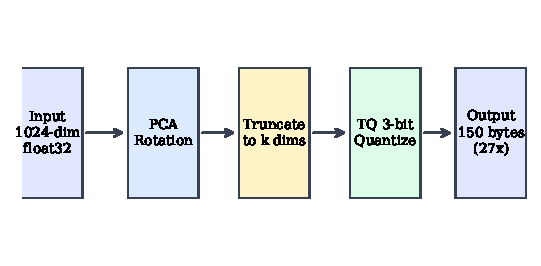
\includegraphics[width=\columnwidth]{fig_pipeline.pdf}
  \caption{The PCA-Matryoshka + TurboQuant compression pipeline. (1) A pre-trained PCA rotation matrix (fit once on a corpus sample) rotates input embeddings into the principal component basis. (2) Trailing dimensions are truncated. (3) The remaining dimensions are quantized to 3 bits using TurboQuant. At query time, the query vector undergoes the same rotation and truncation before search.}
  \label{fig:pipeline}
\end{figure}


% ---- Acknowledgments ----
\section*{Acknowledgments}
The author thanks the San Jos\'{e} State University High-Performance Computing Center for compute resources.
The cross-civilizational ethics corpus was developed as part of the Theory Radar project.


% ---- References ----
\bibliographystyle{IEEEtran}
\bibliography{references}

% ---- Biography ----
\begin{IEEEbiography}[]{Andrew H. Bond}
received the B.S. and M.S. degrees in computer engineering from San Jos\'{e} State University, San Jos\'{e}, CA, USA. He is currently a Lead Consultant at AT\&T and an independent researcher in artificial general intelligence and cognitive architectures. His research interests include embedding compression, geometric reasoning, and cross-civilizational computational ethics.
\end{IEEEbiography}

\end{document}
